\documentclass[border=15pt]{standalone}
\usepackage{tikz}
\usetikzlibrary{calc}

\begin{document}
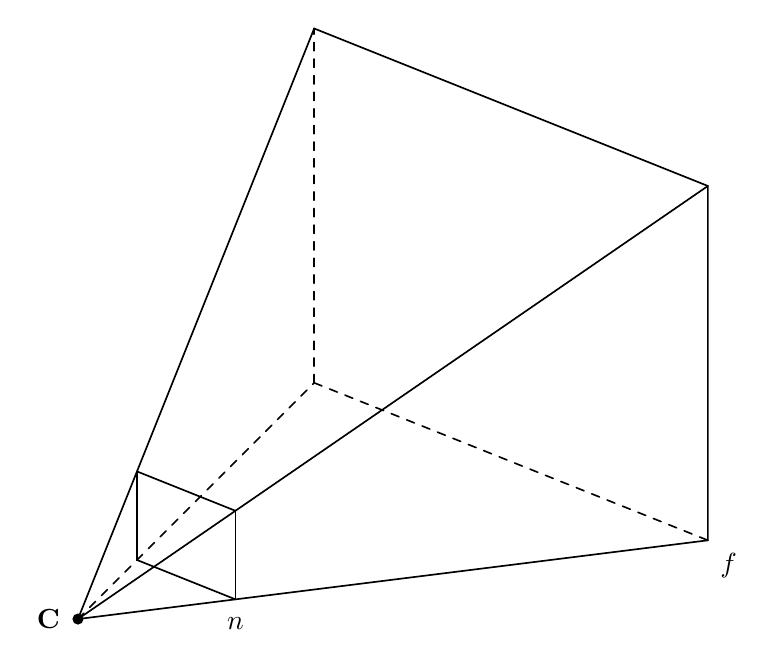
\begin{tikzpicture}[line join=round, line cap=round]

    % Define Center/Apex Point C
    \coordinate (C) at (0,0);
    
    % Define Far Plane coordinates (Calculated as a perfect parallelogram to match the image)
    \coordinate (FBL) at (3, 3);
    \coordinate (FBR) at (8, 1);
    \coordinate (FTL) at (3, 7.5);
    \coordinate (FTR) at (8, 5.5);
    
    % Define Near Plane coordinates (Scaled 25% from C)
    \coordinate (NBL) at ($(C)!0.25!(FBL)$);
    \coordinate (NBR) at ($(C)!0.25!(FBR)$);
    \coordinate (NTL) at ($(C)!0.25!(FTL)$);
    \coordinate (NTR) at ($(C)!0.25!(FTR)$);

    % 1. Draw dashed lines for hidden back edges
    \draw[dashed, semithick] (C) -- (FBL);
    \draw[dashed, semithick] (FBL) -- (FTL);
    \draw[dashed, semithick] (FBL) -- (FBR);



    % 3. Draw visible far plane edges
    \draw[semithick] (FTL) -- (FTR) -- (FBR);

    % 4. Draw near plane
    % Filled with white to occlude the dashed line passing behind it
    \filldraw[fill=white, draw=black, semithick] (NTL) -- (NTR) ;
    \filldraw[fill=white, draw=black, semithick] (NTR) -- (NBR);
    
    \filldraw[fill=white, draw=black, semithick] (NBR) -- (NBL);
    \filldraw[fill=white, draw=black, semithick] (NTL) -- (NBL);
    
    % 2. Draw visible rays from C to far plane corners
    \draw[semithick] (C) -- (FTL);
    \draw[semithick] (C) -- (FTR);
    \draw[semithick] (C) -- (FBR);
    
    % Draw the diagonal cross inside the near plane
    % \draw[semithick] (NTL) -- (NBR);
    % \draw[semithick] (NTR) -- (NBL);

    % 5. Draw the camera point and labels
    \fill (C) circle (2pt);
    \node[left=3pt] at (C) {\textbf{C}};

    % Math labels for planes
    \node[below=3pt] at ($(NBL)!1!(NBR)$) {$n$};
    \node[below right=1pt] at (FBR) {$f$};

\end{tikzpicture}
\end{document}